\begin{tikzpicture}[
    every node/.style={transform shape},
    pinlabel/.style={
        draw=#1!90!black,
        fill=white,
        fill opacity=0.95,
        text opacity=1.0,
        line width=1.1pt,
        rounded corners=3pt,
        font=\sffamily\bfseries\scriptsize,
        text=#1!90!black,
        inner sep=3pt,
        align=center
    },
    pindot/.style={
        circle,
        fill=#1!90!black,
        draw=white,
        line width=1.2pt,
        inner sep=2pt
    },
    pinline/.style={
        draw=#1!90!black,
        line width=1.3pt,
        line cap=round,
        line join=round
    }
]
    % --- Hintergrundbild (PC mit geöffnetem Gehäuse) ---
    \node[anchor=south west, inner sep=0pt, draw=black!70, line width=1pt, rounded corners=2pt] (img) at (0,0) {
        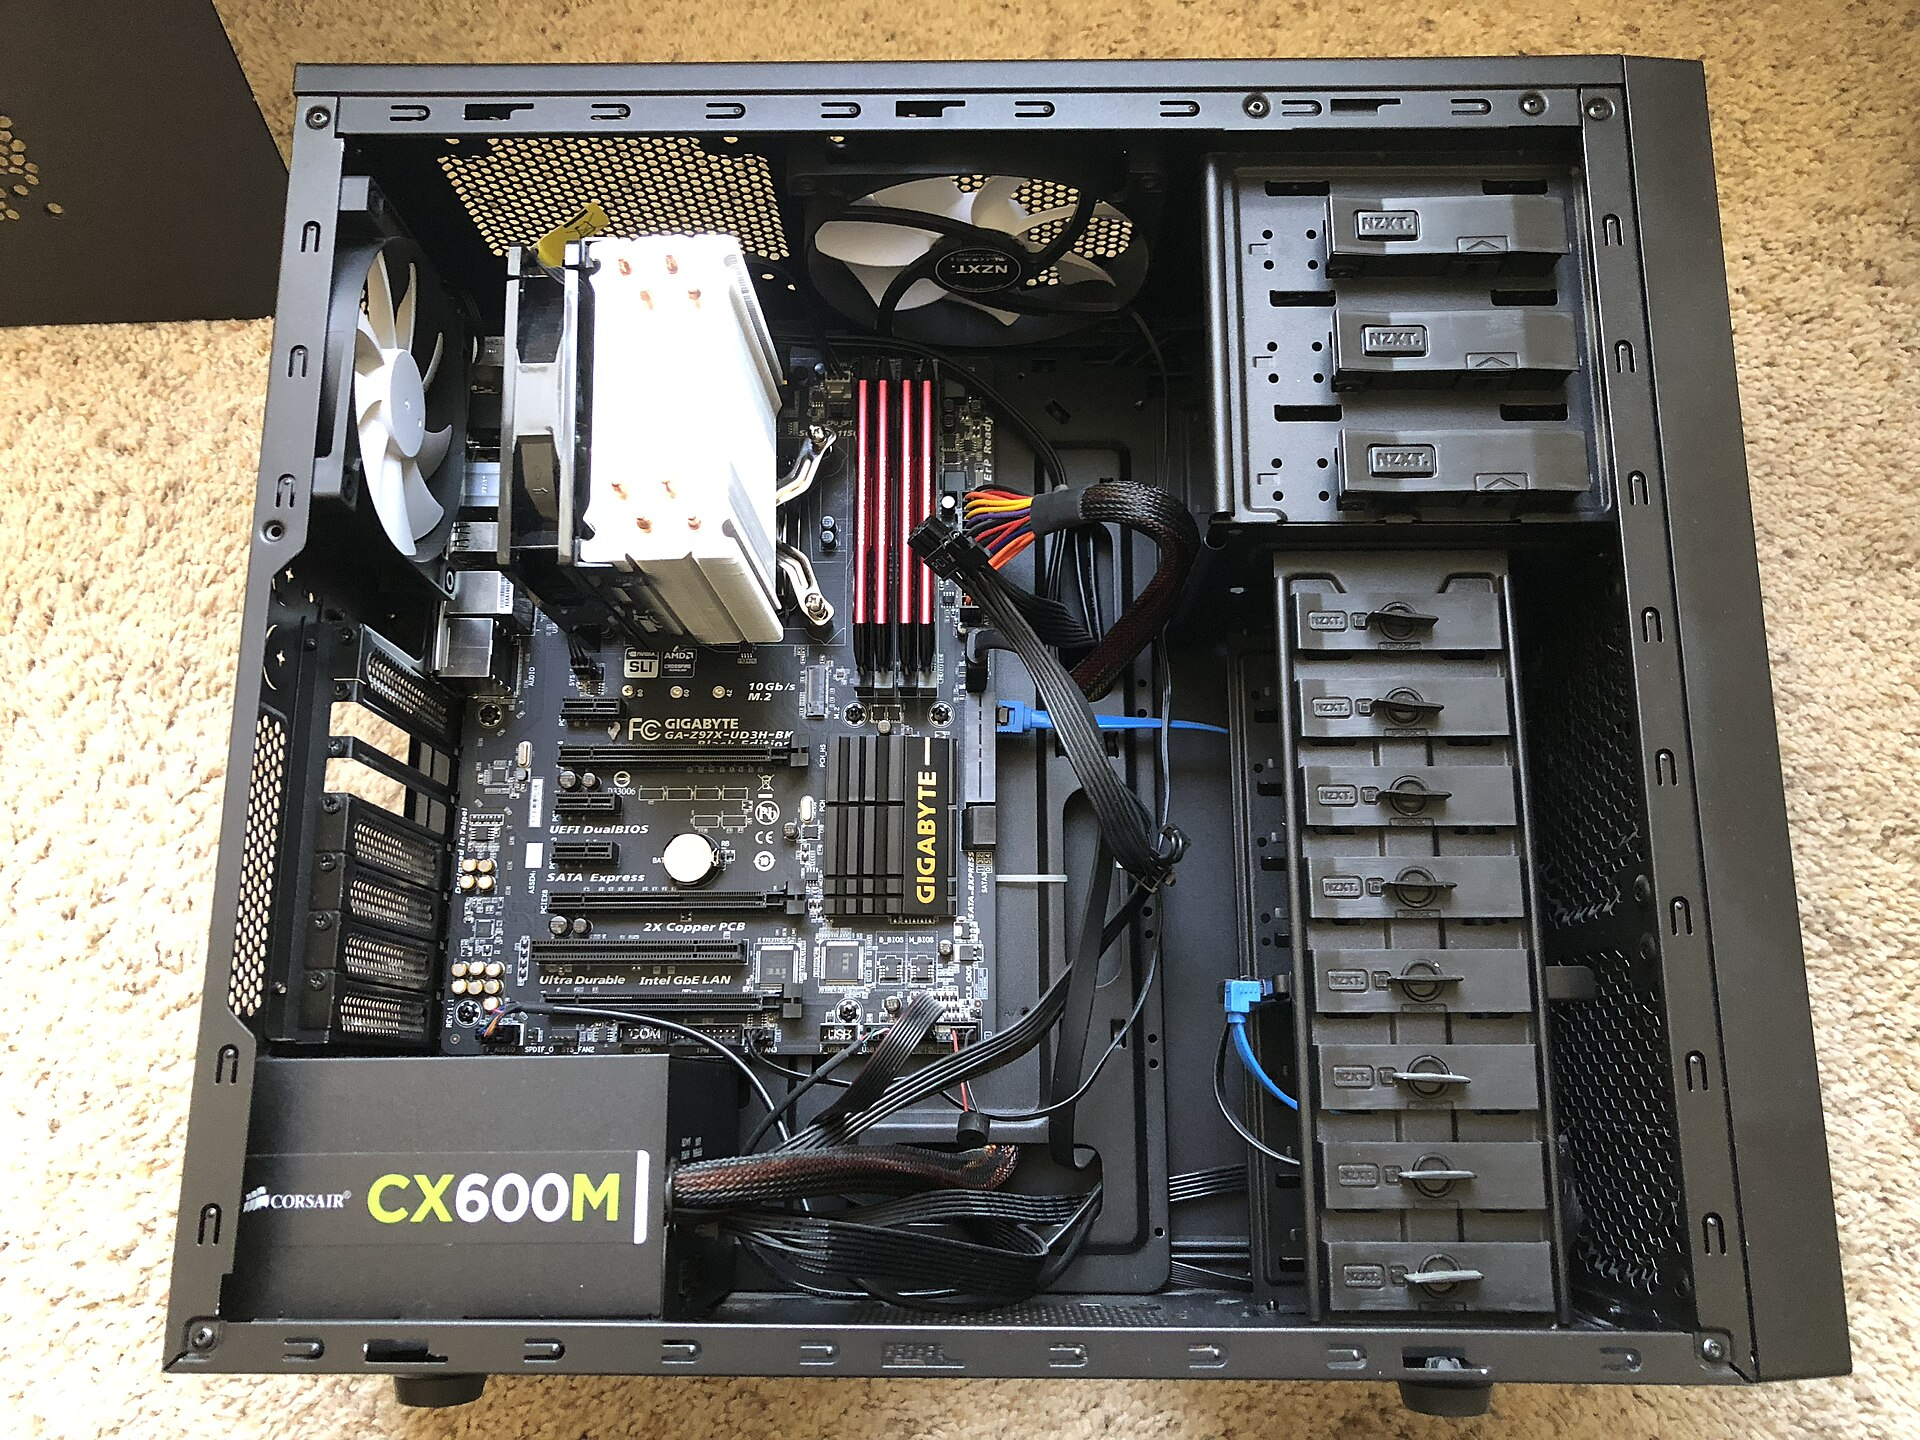
\includegraphics[width=\linewidth]{Grundlagen_Info/16_ComputerUndKodierungen/Figures/pc_inside.jpg}
    };

    % --- Normalisiertes Koordinatensystem (0..1) über dem Bild ---
    \begin{scope}[x={(img.south east)}, y={(img.north west)}]

        % 1. CPU / CPU-Kühler & Sockel (Oben Links)
        \coordinate (cpu_target) at (0.35, 0.72);
        \coordinate (cpu_label) at (0.24, 0.96);
        \draw[pinline=ForestGreen] (cpu_target) -- ++(-0.04, 0.12) -- (cpu_label);
        \node[pindot=ForestGreen] at (cpu_target) {};
        \node[pinlabel=ForestGreen, anchor=north] at (cpu_label) {\glsentryshort{CPU}-Kühler\\(\glsentryshort{CPU} \& Sockel darunter)};

        % 2. Arbeitsspeicher / RAM (Oben Rechts)
        \coordinate (ram_target) at (0.465, 0.70);
        \coordinate (ram_label) at (0.64, 0.96);
        \draw[pinline=Teal] (ram_target) -- ++(0.06, 0.14) -- (ram_label);
        \node[pindot=Teal] at (ram_target) {};
        \node[pinlabel=Teal, anchor=north] at (ram_label) {Arbeitsspeicher (\glsentryshort{RAM})\\(4$\times$ \glsentryshort{DIMM}-Riegel)};

        % 3. I/O-Panel (Links Oben)
        \coordinate (io_target) at (0.25, 0.68);
        \coordinate (io_label) at (0.04, 0.68);
        \draw[pinline=Salmon] (io_target) -- (io_label);
        \node[pindot=Salmon] at (io_target) {};
        \node[pinlabel=Salmon, anchor=west] at (io_label) {I/O-Panel\\(externe Anschlüsse)};

        % 4. Hauptplatine (Mainboard) (Links Mitte)
        \coordinate (mb_target) at (0.33, 0.54);
        \coordinate (mb_label) at (0.04, 0.54);
        \draw[pinline=DarkSlateGray] (mb_target) -- (mb_label);
        \node[pindot=DarkSlateGray] at (mb_target) {};
        \node[pinlabel=DarkSlateGray, anchor=west] at (mb_label) {Hauptplatine\\(Mainboard)};

        % 5. PCIe-Steckplätze (Links Mitte-Unten)
        \coordinate (pcie_target) at (0.34, 0.40);
        \coordinate (pcie_label) at (0.04, 0.40);
        \draw[pinline=RoyalBlue] (pcie_target) -- (pcie_label);
        \node[pindot=RoyalBlue] at (pcie_target) {};
        \node[pinlabel=RoyalBlue, anchor=west] at (pcie_label) {\glsentryshort{PCIe}-Steckplätze\\(für Grafikkarten etc.)};

        % 6. Netzteil / PSU (Links Unten)
        \coordinate (psu_target) at (0.24, 0.17);
        \coordinate (psu_label) at (0.04, 0.22);
        \draw[pinline=DarkSlateGray] (psu_target) -- ++(-0.06, 0.05) -- (psu_label);
        \node[pindot=DarkSlateGray] at (psu_target) {};
        \node[pinlabel=DarkSlateGray, anchor=west] at (psu_label) {Netzteil (\glsentryshort{PSU})\\(Stromversorgung)};

        % 7. 24-Pin ATX Stromanschluss (Rechts Oben)
        \coordinate (atx_target) at (0.52, 0.65);
        \coordinate (atx_label) at (0.96, 0.72);
        \draw[pinline=DarkSlateGray] (atx_target) -- ++(0.12, 0.07) -- (atx_label);
        \node[pindot=DarkSlateGray] at (atx_target) {};
        \node[pinlabel=DarkSlateGray, anchor=east] at (atx_label) {24-Pin ATX\\Stromanschluss};

        % 8. M.2-NVMe Steckplatz (Rechts Mitte)
        \coordinate (m2_target) at (0.41, 0.54);
        \coordinate (m2_label) at (0.96, 0.56);
        \draw[pinline=Orchid] (m2_target) -- ++(0.20, 0.02) -- (m2_label);
        \node[pindot=Orchid] at (m2_target) {};
        \node[pinlabel=Orchid, anchor=east] at (m2_label) {M.2-\glsentryshort{NVMe}-Steckplatz\\(schnelle \glsentryshort{SSD})};

        % 9. Laufwerksschächte (Rechts Unten)
        \coordinate (disk_target) at (0.73, 0.38);
        \coordinate (disk_label) at (0.96, 0.38);
        \draw[pinline=Orchid] (disk_target) -- (disk_label);
        \node[pindot=Orchid] at (disk_target) {};
        \node[pinlabel=Orchid, anchor=east] at (disk_label) {Laufwerksschächte\\(\glsentryshort{SSD}- / \glsentryshort{HDD}-Käfig)};

        % 10. Chipsatz (Mitte Unten)
        \coordinate (chip_target) at (0.48, 0.40);
        \coordinate (chip_label) at (0.48, 0.27);
        \draw[pinline=DarkSlateGray] (chip_target) -- (chip_label);
        \node[pindot=DarkSlateGray] at (chip_target) {};
        \node[pinlabel=DarkSlateGray, anchor=north] at (chip_label) {Chipsatz (Controller)};

    \end{scope}
\end{tikzpicture}
